\documentclass[UTF8]{ctexart}

\usepackage[top=1in,bottom=1in,left=1in,right=1in]{geometry}
\usepackage[raggedright]{titlesec}
\usepackage{hyperref}
\usepackage{bookmark}
\usepackage{graphicx}
\usepackage{tabularx}
\usepackage{makecell}
\usepackage{multirow}
\usepackage{amsmath}
\usepackage{subcaption}
\usepackage{subcaption}
\usepackage{float}

\renewcommand{\thesection}{\chinese{section}.}
\renewcommand{\thesubsection}{\arabic{subsection}}

\graphicspath{{./}}
\newcommand{\img}[2]{\begin{center}\includegraphics[width=#1\textwidth]{#2}\end{center}}
\newcommand{\m}[1]{\,\mathrm{#1}}
\newcommand{\cel}{\,{}^\circ\mathrm{C}}
\newcommand{\abs}[1]{\left\vert{#1}\right\vert}


\title{路径追踪大作业报告}

\author{致理-信计31 褚砺耘}

\begin{document}
    \maketitle
    \tableofcontents
    \newpage

    \section{引言}
    本次大作业基于清华大学 2024 春计算机图形学基础课程框架完成。在下面的功能实现部分中,会优先展示没有通过线下验收而修改或新增的
    功能与其原理、逻辑,之后再展示验收通过的功能。


    \section{功能实现}

    \subsection{NEE}

    \subsubsection{原理}

    NEE 是一种降低渲染噪点、提高收敛速度的技术,核心思想是将渲染方程的结果拆分为:

    $$
    L = L_{dir} + L_{indir}
    $$

    其中 $L_{dir}$ 项对场景内的光源进行显示地采样,而 $L_{indir}$ 项进行均匀半球采样。为了保证能量无偏,如果 $L_{indir}$ 项采样到了
    光源方向,则需要舍弃。基于面积采样的 NEE 单点计算公式为:
    
    $$
    L_{dir} = \sum_{i=1}^{N} \frac{L_e \cdot f_r(w_o, w_i)\cdot \cos \theta_P \cdot \cos \theta_x}{||x - P||^2 \cdot pdfA(x)}
    $$

    其中:

    \begin{itemize}
        \item $f_r$:BSDF

        \item $\cos \theta_P:$ $n_p \cdot w_i$
        
        \item $\cos \theta_x: n_x \cdot (-w_i)$
        
        \item $pdfA: \frac{1}{A}$
    \end{itemize}

    对完美折射或镜面反射材质进行 NEE 是没有意义的,因为采样方向刚好是折射/反射方向的概率是零测度的,这在渲染方程的积分中没有贡献,因此我们的实现仅考虑
    在漫反射材质上的 NEE 表现。

    \subsubsection{执行逻辑}

    在我们的代码中,对每个 shading 点 $P$, 我们实现的 NEE 逻辑为:

    \begin{enumerate}
        \item 遍历光源,从当前光源表面采样一个点 $x$
        \item 构造从当前点 $P$ 指向光源点 $x$ 的方向 $w_i$
        \item 检查是否被遮挡
        \item 如果没有被遮挡,计算该方向上的光照贡献项,加入 $L_{dir}$
        \item 进行均匀半球采样
    \end{enumerate}

    \subsubsection{NEE 效果图}

    如下是一组基础的有/无 NEE 对同一场景的渲染图,其中采样次数均为 100 次。

    \begin{figure}[htbp]
        \centering
        \begin{minipage}[c]{0.45\textwidth}
            \centering
            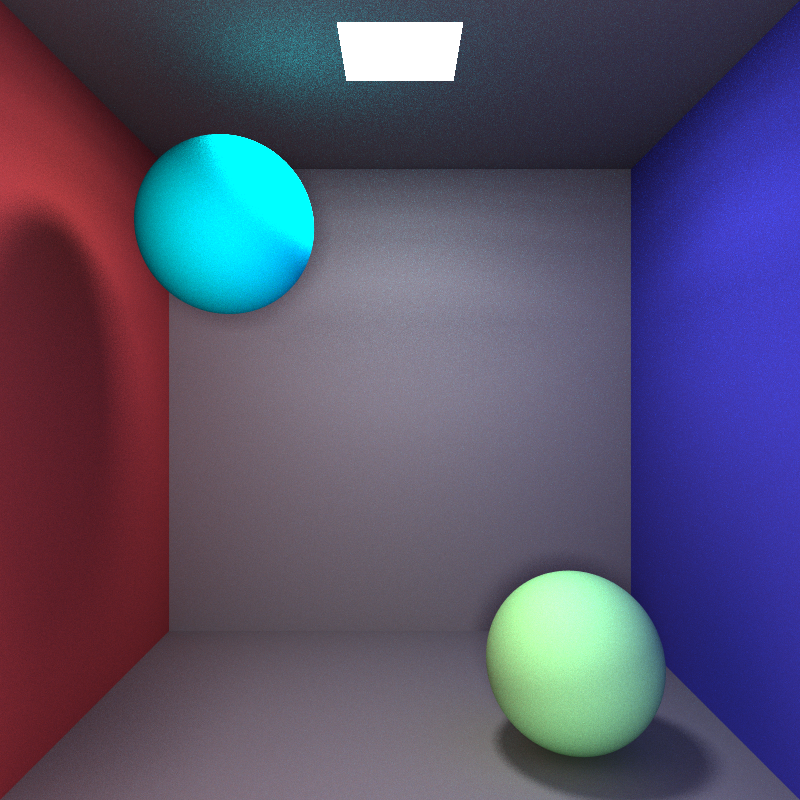
\includegraphics[width=\textwidth]{img/PT_NEE.png}
            \subcaption{NEE}
        \end{minipage}
        \begin{minipage}[c]{0.45\textwidth}
            \centering
            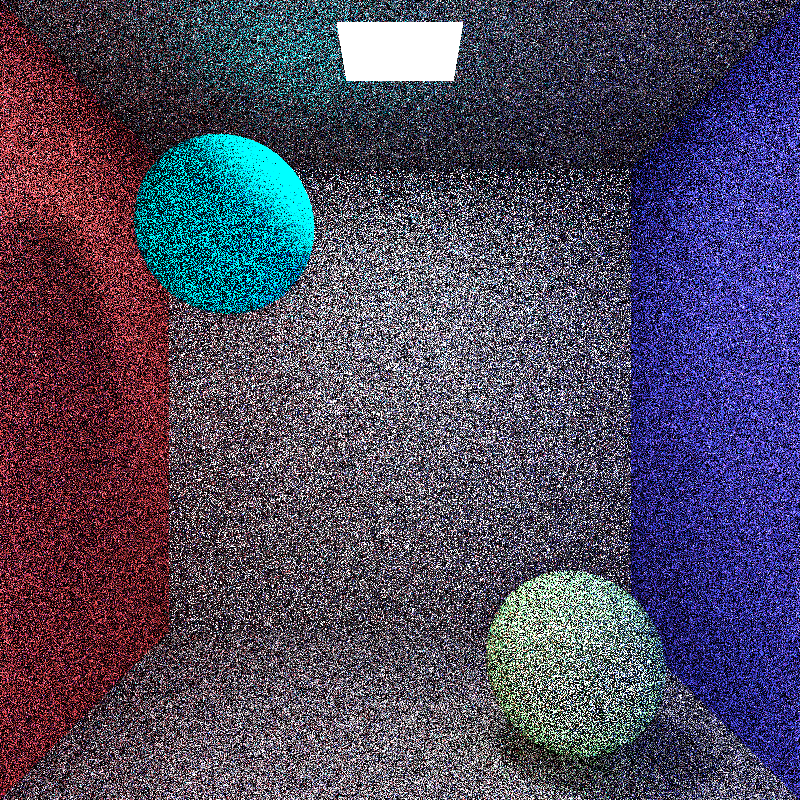
\includegraphics[width=\textwidth]{img/PT_BASIC.png}
            \subcaption{no NEE}
        \end{minipage}
    \end{figure}

    分析图片结果:

    \begin{itemize}
        \item 两张图片的色差一样,代表能量无偏。
        \item NEE在采样100次时已经完全收敛。
        \item 无NEE的PT在采样100次时完全没有收敛,还有极大量的噪点。
    \end{itemize}

    NEE收敛速度明显提升的原因在于,直接对光源进行采样而不是依靠均匀球面采样随机地碰撞到场景内的光源,能够大大提升采样到光源的能力,从而极大程度提高了收敛速度。

    一张 NEE 的最终效果图如下图,考虑到这张图片中有折射和反射材质,而折射和反射不适用NEE,仅采用了最基本的路径追踪,因此需要较大次数的迭代次数确保其收敛。








\end{document}